% XeLaTeX + BibTeX; compile from the repository root into a separate output directory.
\documentclass[11pt,a4paper]{article}
\usepackage{fontspec}
\IfFileExists{C:/Windows/Fonts/times.ttf}{
  \setmainfont{times.ttf}[Path=C:/Windows/Fonts/,BoldFont=timesbd.ttf,ItalicFont=timesi.ttf,BoldItalicFont=timesbi.ttf]
}{\IfFileExists{/mnt/c/Windows/Fonts/times.ttf}{
  \setmainfont{times.ttf}[Path=/mnt/c/Windows/Fonts/,BoldFont=timesbd.ttf,ItalicFont=timesi.ttf,BoldItalicFont=timesbi.ttf]
}{\IfFontExistsTF{Times New Roman}{\setmainfont{Times New Roman}}{\setmainfont{Latin Modern Roman}}}}
\setsansfont{Latin Modern Sans}
\setmonofont{Latin Modern Mono}
\tracinglostchars=3
\usepackage[a4paper,margin=23mm,headheight=15pt]{geometry}
\usepackage{amsmath,amssymb,mathtools,booktabs,tabularx,array,graphicx,xcolor,enumitem,fancyhdr}
\usepackage[numbers,sort&compress]{natbib}
\usepackage[unicode,hidelinks,breaklinks]{hyperref}
\usepackage{xurl}
\setlength{\parindent}{0pt}\setlength{\parskip}{0.45em}\setlength{\emergencystretch}{3em}
\setlist{nosep,leftmargin=1.5em}\renewcommand{\arraystretch}{1.16}
\newcolumntype{Y}{>{\raggedright\arraybackslash}X}
\newcommand{\code}[1]{{\small\nolinkurl{#1}}}
% Shared equations are included by both language editions.
\newcommand{\ScoreEquations}{%
\begin{align}
z_{t,i} &= h_t^{\mathsf T} W_i+b_i,\\
\ell^{\mathrm{full}}_{t,i} &= z_{t,i}-\operatorname{LSE}_{j\in\mathcal V}z_{t,j},\\
\ell^{C}_{t,i} &= z_{t,i}-\operatorname{LSE}_{j\in C_t}z_{t,j}
=\ell^{\mathrm{full}}_{t,i}-\log Q_t(C_t).
\end{align}}
\newcommand{\KLEquations}{%
\begin{align}
p_i^C &= \frac{e^{z_i^S/\tau_S}}{\sum_{j\in C} e^{z_j^S/\tau_S}},\qquad
q_i^C = \frac{e^{z_i^T/\tau_T}}{\sum_{j\in C} e^{z_j^T/\tau_T}},\\
L_C &= \sum_{i\in C}p_i^C\log\frac{p_i^C}{q_i^C},\\
\frac{\partial L_C}{\partial z_j^S} &=
\frac{p_j^C}{\tau_S}\left(\log\frac{p_j^C}{q_j^C}-L_C\right),\quad j\in C.
\end{align}}
\newcommand{\Decomposition}{%
\begin{equation}
D_{\mathrm{KL}}(P\Vert Q) = D_{\mathrm{Ber}}(\alpha\Vert\beta)
+ \alpha D_{\mathrm{KL}}(P^C\Vert Q^C)
+ (1-\alpha)D_{\mathrm{KL}}(P^{\bar C}\Vert Q^{\bar C}).
\end{equation}}
\newcommand{\CounterExample}{%
\begin{equation}
P=(0.49,0.49,0.02),\quad Q=(0.005,0.005,0.99),\quad C=\{0,1\}.
\end{equation}}
\newcommand{\CostEquations}{%
\begin{align}
F_{\mathrm{dense}} &\approx 2RVd, & F_{\mathrm{selected}} &\approx 2RKd,\\
T &\gtrsim \max(F/P_{\mathrm{eff}}, B/\mathrm{BW}_{\mathrm{eff}})
+T_{\mathrm{launch}}+T_{\mathrm{validate}}+T_{\mathrm{pack}},\\
S_{\mathrm{request}} &= \frac{1}{(1-f)+f/s}.
\end{align}}


\hypersetup{pdftitle={Memory-Bounded Teacher Scoring: Contract-Preserving FSDP Integration and Experimental Evidence},pdfauthor={Jiacheng Yu},pdfsubject={AI-assisted technical draft; new content pending Human review}}
\pagestyle{fancy}\fancyhf{}
\fancyhead[L]{\small Memory-bounded teacher scoring}
\fancyhead[R]{\small Human review pending}\fancyfoot[C]{\thepage}
\begin{document}
\hypersetup{pageanchor=false}
\begin{titlepage}
\vspace*{11mm}{\small\sffamily\bfseries AI INFRASTRUCTURE / EXPERIMENTAL TECHNICAL REPORT}\par
\vspace{14mm}{\LARGE\bfseries Memory-Bounded\\[2mm]Teacher Scoring\par}
\vspace{6mm}{\large Contract-preserving FSDP integration, allocator-bounded capacity and direct Worker-to-Student evidence\par}
\vspace{9mm}\hrule\vspace{7mm}
\begin{tabularx}{\linewidth}{@{}p{39mm}Y@{}}
Author & Jiacheng Yu\\
Edition & 30 October 2026; English\\
Document status & AI-assisted technical draft; all new content pending Human review\\
Evidence snapshot & Base \code{0fd56a6}, with the subsequent recorded Worker and mask checks\\
Verified scope & Single-GPU Qwen2/FSDP2; bounded numerical, capacity and restricted-update experiments\\
\end{tabularx}
\par\vspace{9mm}\textbf{Review boundary.} This is a new report. It does not inherit the author-review status of the earlier \code{c1ab1f4} report editions. Those historical reports and the 30 October Markdown/PDF supplement remain separate snapshots. Section~\ref{sec:pending} reports the subsequent bounded Worker and mask checks with their actual measurement limits.
\vfill{\small Measured allocation is reported with its allocator and execution scope. Row chunking is established prior art; this report claims no new selected-logit kernel or general latency improvement.}
\end{titlepage}
\hypersetup{pageanchor=true}

\section*{Abstract}
A compact teacher response can still require an entire token-by-vocabulary logits allocation. This implementation moves row chunking before a Qwen2 LM head while retaining full-vocabulary-normalized scores at Student candidate IDs and the Teacher's own Top-$K$ IDs. The adapter runs inside the ordinary outer FSDP forward, preserves module hooks and tied parameters, and uses native dense forward when an unbudgeted tile covers every projected row. A controlled single-GPU factorial study completed 384 direct-model calls and 64 actual Worker calls without reproducing an earlier CUDA abort. Under a PyTorch allocator fraction of 0.25, the offload-on dense path passed at 1536 rows and failed at 2048, while chunked execution reached 32768; same-length dense correctness was checked only through 8192. At fraction 0.50, dense passed at 8704 and failed at 9216; a higher-budget dense reference confirmed the chunked 9216-row output. Actual Worker outputs also preserved the pinned loss, checked gradients and one final-RMSNorm AdamW update. A later real Worker check matches the complete compact output at 8192 rows, and at 9216 against a higher-budget reference. A separate no-fraction 1024-row check measures memory, not maximum capacity. Full RL training and Ray dispatch remain outside the recorded evidence.
\tableofcontents\clearpage

\section{Motivation and contribution boundary}
Distillation consumers require different information: selected logits, conditional probabilities, full-vocabulary log-probabilities and Teacher Top-$K$ are distinct contracts. An interface returning only $NK$ values does not imply that its implementation avoids an $NV$ projection or allocation. Here $N$ is the number of model rows actually projected, $V$ vocabulary size and $K$ candidate width; padded rows count toward $N$.

Existing per-row scoring interfaces and indexed selected-logit primitives already address parts of this problem. The earlier source survey found relevant SGLang and vLLM interfaces and IndexedLogits; those observations remain tied to their recorded revisions.\cite{sglang38119,vllm56984,indexedlogits,omnilens2026} The engineering subject of this report is narrower: preserving the complete pinned verl Teacher contract while bounding the logits tile in its Qwen2/FSDP execution. Row chunking is an established method, and the selected-logit-only fusion proposal remains \textbf{NO-GO} for this complete contract.

The target is \href{https://github.com/verl-project/verl/tree/87cd055e872f9fdd7b976fcd797a0934b6dba265}{verl PR \#6920 at the fixed revision}\cite{verl6920pinned} \code{87cd055e872f9fdd7b976fcd797a0934b6dba265}. The patch is opt-in; its disabled branch retains the upstream behavior. Source observations and the present local runs do not establish upstream acceptance.

\section{Complete scoring and consumer contract}
For row $t$, let hidden state $h_t$, head weight $W$, bias $b$, and candidate support $C_t$ define:
\ScoreEquations
The returned candidate values are $\ell^{\mathrm{full}}_{t,i}$, not $\ell^C_{t,i}$. The second output is the Teacher's own Top-$K$ over its complete vocabulary. Omitting unselected logits prevents reconstruction of the full normalizer in general; it also fails to determine Teacher Top-$K$. Computing only the Student candidate projection therefore cannot substitute for this two-output interface.

$C_t$ denotes a mathematical support set in these equations. The actual wire carries ordered int64 IDs with shape $[B,T,K]$, can contain repeated IDs, and must preserve that order and multiplicity in gathered scores. Candidate IDs already address causal-logit rows. The adapter adds neither a next-token shift nor a temperature transformation.

The patched Worker still returns exactly \code{teacher_on_student_logp} and \code{teacher_topk_ids} as detached CPU nested tensors in the original valid-row order and with unchanged offsets. Padded candidate IDs are scattered using the actual prepared attention mask and valid rows are restored through that same mask. Multi-sequence padded inputs are supported by this layout path; multi-sequence packed/remove-padding attention is rejected pending verified varlen execution.

For context, support-normalized reverse KL has the fixed-support form:
\KLEquations
This analytical expression explains why the full normalizer cancels after conditional renormalization. It is not a declaration that all OPD losses, clamps or masks implement the same objective. Conditional KL omits support mass and tail structure:\Decomposition
The actual consumer check in Section~\ref{sec:i1} uses the pinned \code{compute_reverse_kl_topk} source, including its configured normalization and clamps, rather than replacing it with this simplified formula. The original source survey distinguished this objective from other OPD reward and subset-loss constructions.\cite{verl6676,opdauthorcode,subsetkl}

\section{FSDP execution and bounded readout}
\subsection{Module and hook lifecycle}
The adapter is installed on the ordinary unwrapped \code{Qwen2ForCausalLM} before FSDP wrapping. It retains the parameter objects, module tree and tied input/output weight. A scored request enters \code{self.engine.module(...)} through the ordinary outer FSDP call. Inside that call, the backbone and final norm run once; flattened hidden rows then enter \code{self.lm_head(tile)} as a module for each tile. Calling the module preserves its own pre/post hooks; directly multiplying its weight would bypass that lifecycle.

For a tile of at most $B$ rows, logits are promoted to FP32 for vocabulary log-sum-exp and candidate gather; scores are cast back to the logits dtype and Teacher Top-$K$ IDs are retained. Tiles are discarded without concatenating full logits. Compact output storage remains proportional to $NK$; the backbone hidden state and model/FSDP allocations remain part of the complete forward.

The verified target is tied-embedding Qwen2 with an ordinary dense linear head, BF16, world size one, eval/no-grad and no KV cache. Adapter guards reject unsupported multi-rank, untied-head, LoRA, quantized/QAT, Liger/fused alternative-forward and sequence-parallel configurations. FP32 code paths are not equivalent to a verified FP32 GPU experiment. FSDP1, TP and multi-GPU support remain \code{NOT_RUN}.

\begin{figure}[htbp]\centering
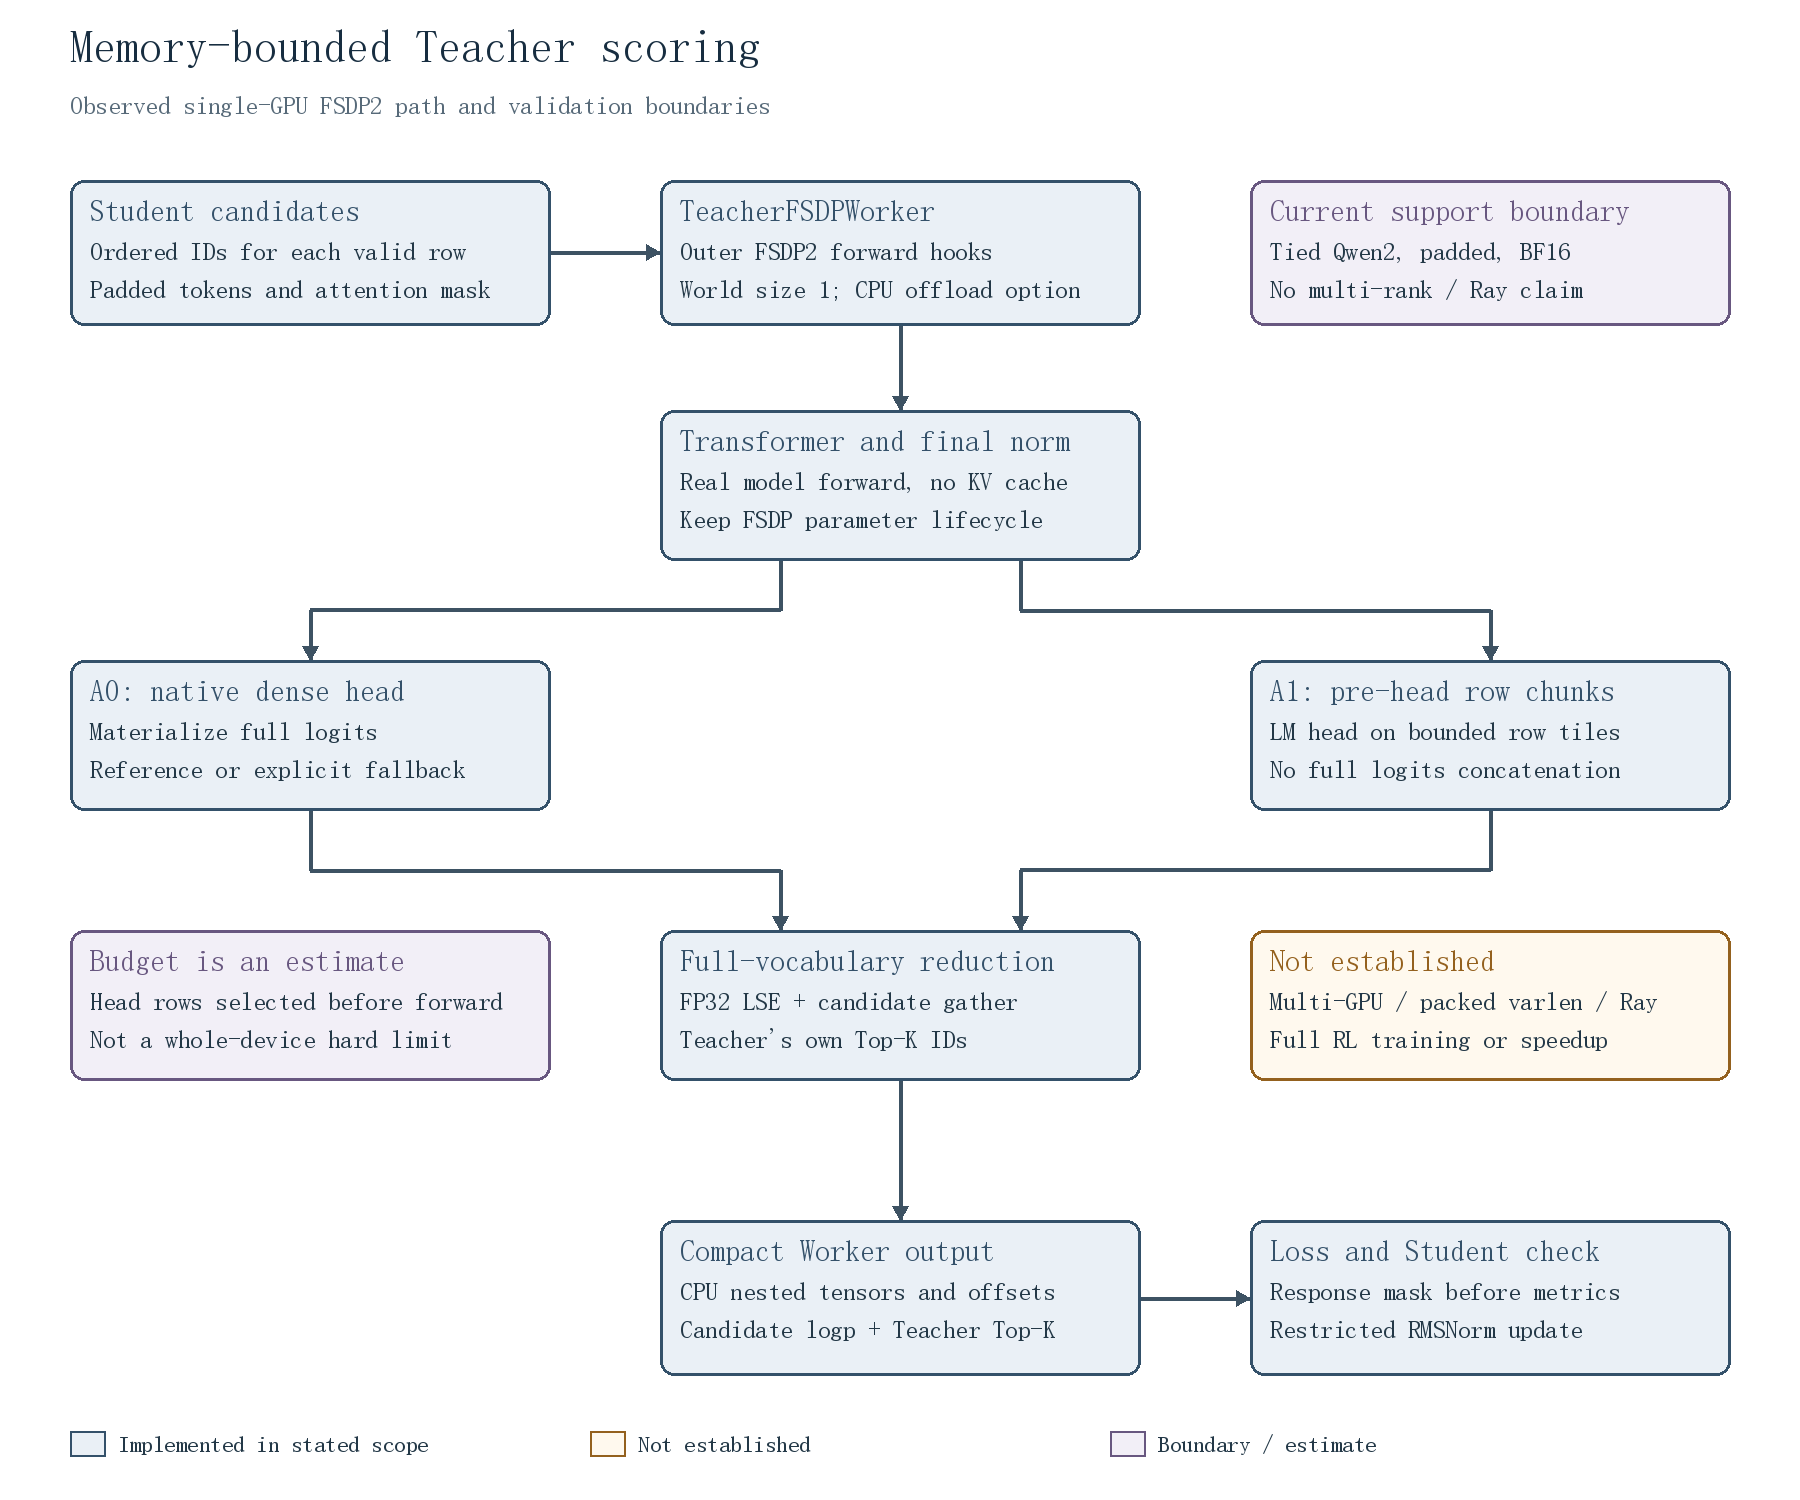
\includegraphics[width=0.98\linewidth,height=0.66\textheight,keepaspectratio]{docs/architecture/memory-bounded.en.png}
\caption{Memory-bounded Teacher execution and the separate direct Worker-to-Student validation path. Numerical and runtime scope is given by the experiment sections; the figure is not evidence of unrun dispatch or training paths.}\label{fig:arch}
\end{figure}

\subsection{CPU offload and dense fallback}
FSDP2 CPU offload changes parameter residency and can dominate complete-forward timing; it does not remove the need to preserve ordinary FSDP forward boundaries. The controlled study inspects actual root/decoder offload policies instead of inferring them from a command-line flag.

With no explicit head budget, a selected tile covering all projected rows invokes \code{dense_full_row_fallback}: native dense forward returns first, and the existing gather/reduction runs outside FSDP. A full-row tile reduced while parameters remain resident can increase the peak; at $N=512$, a full-row chunk of 512 increased an earlier absolute peak by about 33.7\%. This observation motivated the native fallback. Any explicit head budget disables that automatic fallback, so a requested estimate is not silently replaced by unbounded dense execution. Errors and OOM propagate; the outer forward is not retried.

\subsection{Budget estimate and its limits}
Let $s$ be logits element bytes, $\gamma=1.25$ the default safety factor and $H$ the requested head allowance in bytes. The implemented estimate is
\begin{align}
M_{\mathrm{compact}}&=NK(s+8),\\
m_{\mathrm{row}}&=\left\lceil\gamma\,[V(s+8)+24K]\right\rceil,\\
\widehat M(B)&=M_{\mathrm{compact}}+Bm_{\mathrm{row}},\\
B&=\min\!\left(N,B_{\mathrm{requested}},\left\lfloor\frac{H-M_{\mathrm{compact}}}{m_{\mathrm{row}}}\right\rfloor\right).
\end{align}
The estimate includes compact output storage, a logits tile, up to two FP32 vocabulary-sized work tensors and conservative Top-$K$ bookkeeping. If one estimated row plus compact outputs cannot fit, admission fails before the forward. The cap is on this readout estimate, not full-model memory, FSDP residency, fragmentation, other processes or all CUDA workspaces. It leaves full-vocabulary projection work approximately $2NVd$; smaller tiles trade allocation against additional head calls.

An earlier separate $N=1024,K=32$ FSDP2 probe selected 35/70/141 rows for 64/128/256 MiB estimated budgets. Observed readout allocated increments were approximately 51.03/101.75/204.64 MiB; complete-forward peaks were about 552.28 MiB. These observations calibrate that workload only. A head estimate and \code{torch.cuda.set_per_process_memory_fraction} constrain different quantities.

\section{Experimental design and execution identity}
\begin{table}[htbp]\centering\small
\begin{tabularx}{\linewidth}{@{}p{34mm}Y@{}}\toprule
Item & Fixed recorded condition\\\midrule
GPU & NVIDIA RTX 5070 Laptop; 8151 MiB\\
Model & Qwen2.5-0.5B-Instruct; BF16; tied embeddings\\
Model revision & \code{7ae557604adf67be50417f59c2c2f167def9a775}\\
Framework & PyTorch 2.14.1+cu130; Transformers 5.19.0\\
Distributed path & FSDP2, world size one; offload condition recorded separately\\
Input & Synthetic tokenized sequences and fixed candidate IDs; no sampled RL trajectories\\
Evidence source & Bilingual 30 October stage supplement and earlier bounded-adapter records\\\bottomrule
\end{tabularx}\caption{Execution identity for the recorded experiments.}\label{tab:identity}
\end{table}
Capacity points use separate new processes, SDPA, $K=32,B=256$, and a single sequence. The factorial fixture instead uses padded lengths 64/37, $K=8,B=16$ and eager attention. These workloads are not interchangeable. Output signatures cover shape, dtype, offsets and bytes; capacity comparisons inspect all saved compact candidates and Teacher Top-$K$ sets. The comparator preserves unresolved tie/mismatch status when compact outputs alone cannot establish a full-logits boundary tie.

\subsection{Worker-aligned buffer construction}
The first direct-model construction differed numerically from the actual Worker. The pinned Worker explicitly calls \code{model.to(dtype)}, casting Qwen2 rotary frequency buffers from FP32 to BF16; the original direct path retained FP32 buffers. Matching that single construction step changed 31/32 frequency values and restored exact equality on all 808 candidate values and 101 Teacher Top-$K$ rows in the tested fixture. This explains that path difference, not the CUDA abort. Earlier direct-model measurements remain scoped to their recorded buffer policy.

\section{S1: controlled stability}
The direct-model factorial crosses Dense/Chunked with CPU offload on/off. Each condition uses three fresh processes, two warmups and 30 counted calls per process. Actual root/decoder FSDP policies match the requested setting. Each completed call is checked against the same compact reference.
\begin{table}[htbp]\centering\small
\begin{tabularx}{\linewidth}{@{}YYrr@{}}\toprule
Entry & Condition & Processes & Calls\\\midrule
Direct Qwen/FSDP2 & Dense, offload on & 3 & 96\\
Direct Qwen/FSDP2 & Chunked, offload on & 3 & 96\\
Direct Qwen/FSDP2 & Dense, offload off & 3 & 96\\
Direct Qwen/FSDP2 & Chunked, offload off & 3 & 96\\
Actual verl Worker & Dense, offload on & 1 & 32\\
Actual verl Worker & Chunked, offload on & 1 & 32\\\bottomrule
\end{tabularx}\caption{Completed calls include warmups: $3(2+30)=96$ per direct condition.}\label{tab:s1}
\end{table}
The direct processes completed 384 checked calls and the two actual Worker processes completed another 64 with per-call hashes and offsets. The initial CUDA \code{unknown error} did not recur in this bounded set. Its cause, including the contemporaneous WSL dxg observations, remains unknown. Repetition establishes only the observed finite run set, not long-term production stability.

\section{Capacity under stated allocator fractions}
The 0.25 fraction corresponds to a nominal 2,129,510,400-byte PyTorch caching-allocator allowance on this device. It is not an all-device hard partition. The boundary scan narrows tested brackets at 512-token resolution; success/OOM points do not prove monotonicity or an exact maximum.
\begin{table}[htbp]\centering\small
\begin{tabularx}{\linewidth}{@{}p{15mm}p{17mm}YYY@{}}\toprule
Fraction & Offload & Dense pass / next OOM $N$ & Chunked largest tested runnable $N$ & Dense-checked chunked through $N$\\\midrule
0.25 & On & 1536 / 2048 & 32768 & 8192\\
0.25 & Off & 512 / 1024 & 16384 / OOM 16896 & 4096\\
0.50 & On & 8704 / 9216 & 32768 & 9216\\\bottomrule
\end{tabularx}\caption{Observed grid points and separate numerical-equivalence boundaries.}\label{tab:capacity}
\end{table}
At fraction 0.25, offload-on compact comparisons passed at $N=1024,2048,4096,8192$ and offload-off comparisons at $N=2048,4096$, with maximum logprob difference zero. Longer Dense references used fraction 0.55; reference attempts at $N=12288$ on and $N=8192$ off OOMed. The corrected comparator reran all six cases after adding shape/signature validation; prior comparison records were retained.

Thus the offload-on 8192/1536 observed length ratio is 5.33, while 32768 remains execution-capacity evidence without full same-$N$ Dense correctness. At fraction 0.50, Chunked ran at 8192/16384/24576/32768. The $N=8192$ same-budget comparison matched; a fraction-0.55 Dense reference at $N=9216$ matched all 294,912 candidate values and all 9216 Top-$K$ sets from fraction-0.50 Chunked. This verified grid point is 512 tokens (5.88\%) beyond Dense's largest tested 8704 pass. The higher-budget reference supplies correctness, not a same-budget capacity advantage.

\section{M1 and T1: memory scope and descriptive timing}
\subsection{Allocator peaks and whole-device observations}
\begin{table}[htbp]\centering\small
\begin{tabularx}{\linewidth}{@{}Yrrrr@{}}\toprule
Metric, MiB & \multicolumn{2}{c}{$N=1024$, M1} & \multicolumn{2}{c}{$N=8192$, fraction 0.50}\\
 & Dense & Chunked & Dense & Chunked\\\midrule
Forward allocated peak & 1517.09 & 665.31 & 3596.83 & 681.66\\
Process allocator peak incl. load/wrap & 1517.09 & 958.48 & 3596.83 & 958.48\\
Forward reserved peak & 1748 & 1572 & 3846 & 1572\\
Sampled whole-device used max & 3429 & 3258 & 5504 & 3229\\
Device sample count (not MiB) & 40 & 30 & 36 & 33\\\bottomrule
\end{tabularx}\caption{Separate fresh Dense/Chunked processes, offload on. The 100 ms device sampler includes all processes and may miss transient peaks.}\label{tab:memory}
\end{table}
The lower call-only allocator peak does not erase loading/wrapping allocations. Reserved memory also depends on allocator history. The $N=1024$ sampled maxima differ by 171 MiB; that is not an exact process-VRAM saving. At the fraction-0.50 Dense OOM, CUDA still reported approximately 3401 MiB free, identifying an allocator-budget boundary rather than device exhaustion. No unrestricted-allocator long-Worker capacity result is recorded here.

\subsection{Worker-aligned paired forward timing}
T1 uses $N=1024,K=32,B=256$, six A/A blocks and eight interleaved ABBA/BAAB blocks per offload condition, giving 16 samples per A/B label. Loading and correctness validation are outside the timed complete direct-model/FSDP forward; compact CPU copies are inside it.
\begin{table}[htbp]\centering\small
\begin{tabularx}{\linewidth}{@{}p{18mm}Yrr@{}}\toprule
Offload & Metric & A0 Dense & A1 Chunked\\\midrule
On & Allocated peak MiB & 1517.09 & 664.97\\
Off & Allocated peak MiB & 2467.26 & 1615.48\\
On & perf-counter p50 / p95 ms & 192.580 / 193.953 & 192.978 / 198.150\\
On & raw-clock p50 / p95 ms & 190.491 / 191.858 & 190.926 / 196.081\\
Off & perf-counter p50 / p95 ms & 87.241 / 114.847 & 78.709 / 116.953\\
Off & raw-clock p50 / p95 ms & 87.567 / 115.198 & 78.986 / 117.407\\\bottomrule
\end{tabularx}\caption{Recorded direct-model paired measurements with Worker-aligned buffer casting.}\label{tab:timing}
\end{table}
Allocated decreases were 56.17\% on and 34.52\% off in this scope. Both candidate comparisons had maximum difference zero and all 1024 Teacher Top-$K$ sets matched. In the offload-off process, CUDA Event exceeded its surrounding perf-counter span in 30/32 A/B and 12/12 A/A samples. Earlier runs also showed host-clock and phase drift; their cause remains unresolved. Timings remain descriptive, with no general speedup claim and no production comparison across the two separate offload processes.

\section{I1: actual Worker output into a restricted Student update}\label{sec:i1}
A real Qwen Student generates candidates once. Actual pinned \code{TeacherFSDPWorker} objects then execute Dense fallback and Chunked scoring sequentially. Their returned in-memory CPU nested TensorDict values are scattered into the original padded Student rows and passed directly to \code{compute_reverse_kl_topk}. No recorded JSON Teacher values substitute for these outputs.

The two sequences have offsets $[0,23,45]$, 46 padded model rows, $K=8$ and 25 active response-prediction rows. Student selection uses temperature 0.8 followed by log-softmax and Top-$K$; Teacher temperature is 1. Candidates remain on their original logit rows; only the response mask receives next-token alignment. Both paths restore the same final RMSNorm weight and fresh AdamW state, learning rate 0.01 and zero weight decay. Teacher tensors are detached; support normalization, logprob clamp $-10$, nonnegative token-loss clamp and maximum loss clamp 10 are retained.
\begin{table}[htbp]\centering\small
\begin{tabularx}{\linewidth}{@{}Yrr@{}}\toprule
Observed quantity & Dense Worker & Chunked Worker\\\midrule
Masked scalar loss & 0.0216006283 & 0.0216006283\\
Final RMSNorm gradient L2 & 0.0124774044 & 0.0124774044\\
Nonzero gradient elements & 896 & 896\\
Changed BF16 parameter values & 1 & 1\\
Parameter-update L2 & 0.0099792480 & 0.0099792480\\\bottomrule
\end{tabularx}\caption{One final-RMSNorm AdamW update using actual Worker outputs.}\label{tab:i1}
\end{table}
All 360 candidate values, Teacher Top-$K$, mass, overlap, token losses, 6,989,056 Student logits-gradient elements, 896 RMSNorm-gradient elements and resulting updates matched exactly in the fixture. Normal outer/head hook completion, absent Teacher gradients and collection of both sequential Worker Python objects were checked. This establishes local Worker-to-loss-to-restricted-update integration; Ray dispatch, a complete Trainer, all-parameter optimization and an RL step remain \code{NOT_RUN}.

\section{Negative results and evidence interpretation}
The initial selected-logit proposal does not satisfy full normalization plus Teacher Top-$K$. An earlier full-row chunk increased the complete peak and led to the explicit native fallback policy. The initial CUDA abort remains unexplained despite the bounded non-reproduction set. Buffer casting explains one direct/Worker numerical difference but provides no evidence about that abort.

An earlier project-consumer version independently cast BF16 Student logprob to FP32 on two gradient branches. Scalar loss matched upstream, but RMSNorm and logits gradients differed by about 1.07\% and 1.80\% relative L2. Reusing the FP32 conversion as the upstream graph does removed those differences for the fixture. This retained negative result motivates comparing gradients and updates, rather than accepting scalar-loss equality alone.

Earlier transient samples lost after WSL temporary storage was cleared are not reconstructed; later recorded runs form the cited measurement scope. The archived matrix also mislabeled a full-row head call as avoiding full logits; actual call shapes contradicted the label and the current script corrected it. Longer chunked runs beyond the Dense-reference ceiling retain \code{UNKNOWN} numerical equivalence. No report wording converts an exit code or a finite-output run into complete numerical or training acceptance.

\section{Real long Worker, natural allocation and response-mask checks}\label{sec:pending}
These later measurements use the actual pinned \code{TeacherFSDPWorker} in fresh processes, tied Qwen2 BF16, FSDP2 CPU offload, SDPA, $K=32$ and row chunk $B=256$. Text and candidate IDs are synthetic. Every call records actual input, attention mask, position IDs, offsets, outer/backbone/head hooks and the complete CPU nested output. Two short processes with lengths 64/37 exercise real padding; all 3232 candidate logprobs and 101 ordered Teacher Top-$K$ rows match. The long tests each use one causal sequence; they do not establish long multi-sequence padding behavior.

\begin{table}[htbp]\centering\small
\begin{tabularx}{\linewidth}{@{}Yrrrr@{}}\toprule
Worker condition & \multicolumn{2}{c}{Allocated peak, MiB} & \multicolumn{2}{c}{Reserved peak, MiB}\\
 & Dense & Chunked & Dense & Chunked\\\midrule
8192, both fraction 0.50 & 3596.638 & 681.630 & 3844 & 866\\
9216, dense 0.55 / chunked 0.50 & 3893.700 & 683.962 & 4144 & 884\\
1024, no fraction, A/A and B/B & 1517.071 & 665.306 & 2644 & 1124\\\bottomrule
\end{tabularx}\caption{Complete Worker-call allocator peaks in independent processes. The 9216 Dense fraction is a correctness reference, not a same-budget capacity comparison.}\label{tab:worker-release}
\end{table}

At $N=8192$, all 262,144 candidate logprobs and all 8192 ordered Teacher Top-$K$ rows match exactly. At $N=9216$, all 294,912 candidate values and 9216 ordered Top-$K$ rows match exactly across the stated fractions. Each long cell is one cold call; the frozen BF16 tolerance is also satisfied. The matching long outputs have offsets $[0,N]$. These observations do not validate 32768 against dense or establish a full Trainer run.

Without calling \code{set_per_process_memory_fraction}, four new $N=1024$ processes ran in ABBA order, each with one warmup and three measured calls. The recorded actual fraction was 1.0 in each. A/A, B/B and A/B compact outputs matched, including ordered Top-$K$. Dense measured perf-counter samples ranged 175.754--200.623 ms and Chunked 161.573--191.955 ms; host clocks disagreed in some samples. These are descriptive small-sample timings, not an acceleration claim. The 100 ms all-device maximum samples were 4990/5120 MiB for the two Dense processes and 3584/3332 MiB for the two Chunked processes; these include other processes and can miss peaks. No no-fraction capacity ceiling was tested.

The fixed trainer's metric wrapper masks to response rows before mass, loss range and overlap aggregates; overlap advantage additionally requires positive overlap. The local diagnostic now applies the same rules while retaining raw per-token outputs. CPU tests compare with the actual fixed trainer functions and a hand-calculated oracle, including extreme or NaN prompt/padding values and zero-overlap rows; loss and gradient behavior is unchanged. A CPU replay of the prior I1 record retains the padded \code{teacher_mass=8.0} but excludes it: response-only Teacher mass mean is 0.732026 and maximum 0.999786 for 25 response rows. This replay is not a new GPU training step.

Two initial starts were \code{NOT_RUN} because the predeclared free-memory gate was not met; an initial CPU dependency import also failed and the runner was corrected before GPU execution. All ten completed Worker processes report no device-sampler failure. The subsequent probe revision makes a missing device observation fail the experiment while retaining any successful Worker output; the executed probe source and its SHA-256 remain with the raw measurements. This later error-handling correction was CPU-regression-tested and does not retroactively change the recorded runs.

\section{Final bounded Worker comparison}
The final matrix used the same pinned Worker and Qwen2.5 BF16 fixture with $K=32$, SDPA, FSDP2 CPU offload and allocator fraction 0.50. For each of $N=1024,4096,8192$, four fresh processes ran Dense--Chunked--Chunked--Dense; each process had one first-call warmup and five measured calls. All 96 saved compact outputs, including warmups and the chunk-size sweep, were reloaded and compared against their same-length Dense references. Candidate logprobs and ordered Teacher Top-$K$ were exact in this matrix.

\begin{table}[htbp]\centering\small
\begin{tabularx}{\linewidth}{@{}rYrrrr@{}}\toprule
$N$ & Mode & Alloc. MiB & Reserv. MiB & p50 ms & p95 ms\\\midrule
1024 & Dense & 1517.1 & 2644 & 210.4 & 288.0\\
1024 & Chunked & 665.3 & 1124 & 159.4 & 187.0\\
4096 & Dense & 2409.4 & 2944 & 322.3 & 414.4\\
4096 & Chunked & 672.3 & 1130 & 318.8 & 327.5\\
8192 & Dense & 3596.6 & 3846 & 570.8 & 599.6\\
8192 & Chunked & 681.6 & 1126 & 626.3 & 944.6\\\bottomrule
\end{tabularx}\caption{Per-call PyTorch allocator peaks and warmed, synchronized Worker spans; $B=256$. Each mode/length has 10 measured samples across two processes. Percentiles use linear interpolation.}\label{tab:final-matrix}
\end{table}

\begin{figure}[htbp]\centering
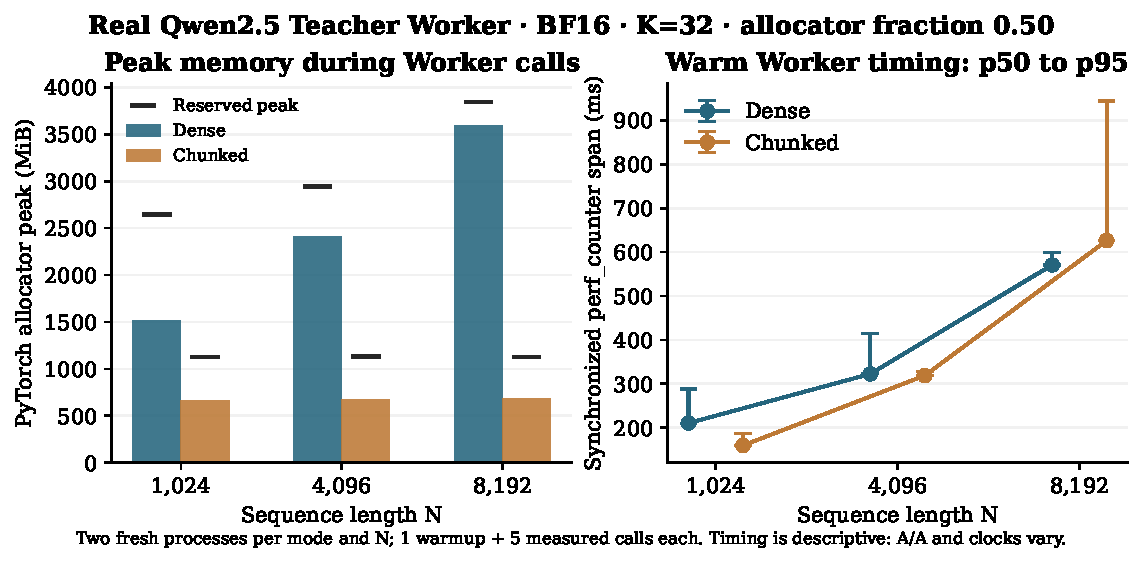
\includegraphics[width=\linewidth]{docs/figures/worker-memory-timing.pdf}
\caption{Measured allocator peaks and descriptive Worker timing. Reserved markers are PyTorch reserved peaks; they are not total-device memory.}\label{fig:final-memory}
\end{figure}

The $N=8192$ allocated peak decreased by 81.05\% in this measured Worker-call scope. In the same allocator fraction, Dense succeeded at 8704 and OOMed at 9216, while Chunked succeeded at 16384 and 32768. These are tested points, not proof of the exact maximum or total-device exhaustion; no same-length Dense oracle exists at 32768. Start/end device snapshots were recorded, but an exact all-device peak was not measured.

\begin{figure}[htbp]\centering
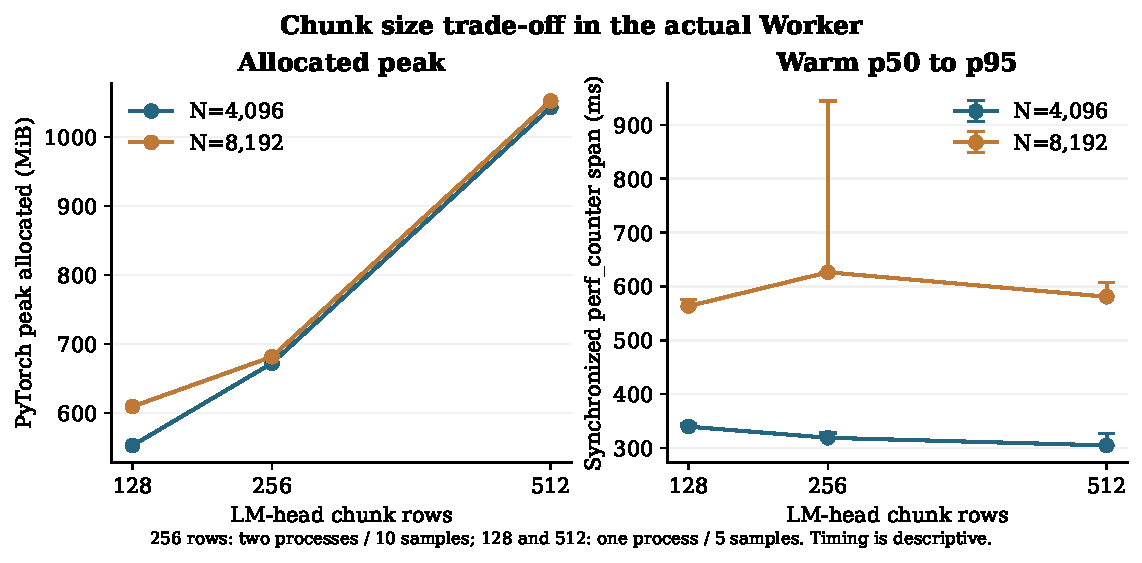
\includegraphics[width=\linewidth]{docs/figures/worker-chunk-tradeoff.pdf}
\caption{Chunk-size sensitivity. The 256-row point has two processes and 10 samples; 128 and 512 each have one process and five samples.}\label{fig:chunk-tradeoff}
\end{figure}

\begin{samepage}
Latency is descriptive: the two $N=1024$ Dense process medians were 229.2 and 158.0 ms, and a chunk-sweep sample showed an 8.33\% host-clock difference. An earlier single cold $N=8192$ pair measured 3382.176 ms Dense and 8756.047 ms Chunked. The synchronized cold spans run through nested CPU return and include diagnostic hooks and sampling; they do not establish a stable slowdown. The initial CUDA error and the clock discrepancies remain unexplained; no general speedup is claimed. In separate one-call $N=4096$ profiler captures, Dense / Chunked recorded 97 / 112 \code{aten::mm} calls (88.8 / 103.6 ms self CUDA), one / 16 \code{aten::topk} calls (18.0 / 19.7 ms self CUDA) and 290 pinned host-to-device copies each (74.9 / 73.3 ms of recorded device intervals). Matrix multiplication, transfers and reduction all contribute to the observed work. These categories may overlap or be nested, and profiling adds overhead; their durations must not be summed as the critical path or treated as an unprofiled latency result.\par
\end{samepage}

The existing actual Worker-to-Student test compared the pinned reverse-KL loss, gradients and a restricted RMSNorm update. An additional CPU replay compared that actual upstream loss and Student-logits gradients for 16 sampled rows at each length using synthetic candidate IDs. It is not a real Student trajectory or complete RL training.

\section{Reproduction and final technical judgment}
A separate clean scoring checkout at \code{0273017} received the package-import fix, and a new Python 3.12 environment was installed from the 105-package hash lock. A separately downloaded pinned model was hash-checked, and real Dense and Chunked N=1024 Workers returned 32,768 exactly matching candidate values and 1024 ordered Top-K rows. The clean checkout ran 195 tests with CUDA enabled; the final working tree including the additional sampler regression ran 199. The earlier dependency and import failures remain in the private experiment evidence. The public \code{results/worker-evidence-manifest.json} binds archived raw artifacts by SHA-256; the archive itself remains in the private project workspace.\par


The base source snapshot is \code{0fd56a618800b5298d8c45529dda675f910c6e47}; the later Worker probe and mask regression are in the revision containing this report. The raw records bind the probe bytes used for the measured runs. The pinned loss is \href{https://github.com/verl-project/verl/blob/87cd055e872f9fdd7b976fcd797a0934b6dba265/verl/trainer/distillation/fsdp/losses.py}{the actual verl FSDP distillation loss}, Git blob \code{97d3ebf485a5ce9e1b1a435cce427d6d89284dc6}. Model and tokenizer hashes, command arguments and source identities accompany the original measurements.

The principal entries include \code{scripts/long_worker_probe.py}, \code{scripts/factorial_teacher_probe.py}, \code{scripts/compare_capacity_outputs.py}, \code{scripts/full_teacher_benchmark.py} and \code{scripts/worker_to_student_step.py}. Evidence identifiers include \code{S1_SUMMARY.json}, \code{capacity_runner.jsonl}, \code{compare_validated_summary.json}, \code{compare_on_n9216.json}, \code{T1_worker_aligned_on/off.json} and \code{worker_to_student_01.json}. The bilingual Markdown stage supplement supplies the preceding measured tables; the later section above uses the recorded Worker runs and CPU mask regression.

The supported conclusion is contract-preserving bounded readout with measured allocator-capacity benefits and a real restricted consumer update in the stated single-GPU environment. FP32 GPU, FSDP1, TP/multi-GPU, packed varlen, LoRA/quantization/QAT, Ray transport, representative RL trajectories, full-model training and production stability remain unverified. General latency improvement, exact total-device VRAM savings and training-quality gains are not established. All new text remains AI-assisted and pending Human review.

\clearpage
\bibliographystyle{plainnat}
\bibliography{docs/reports/references}
\end{document}
